\section{System Management Mode (\gls{smm})}\label{section-smm}
\subsection{Overview}
On \say{IA-32 processors}, System Management Mode (\gls{smm}) is a manner of operation which is different from flat modal so as from protected mode of the DXE and PEI phases. It is outlined as a real mode environs with $ 32-bit $ data bus access and its carried out in effect to either with a specified interrupt type or with the System Management Interrupt (\gls{smi}) pin. Note that Operation mode of SMM is OS independent mode and is discrete operational mode, however it may also lies in both within and OS runtime.

\begin{figure}[!htbp]
	\centering
	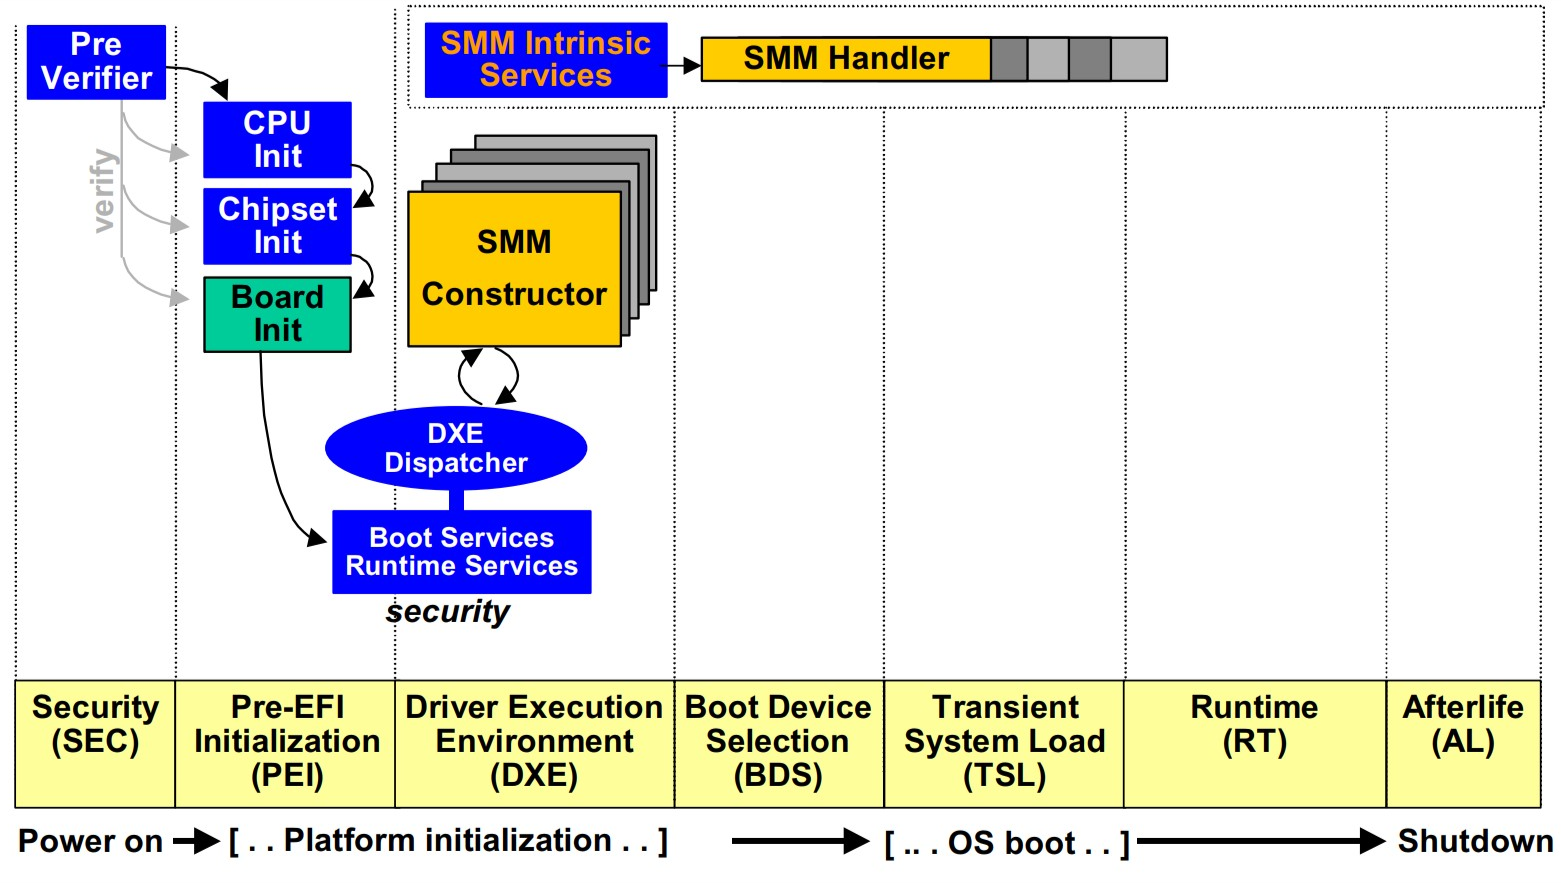
\includegraphics[width=0.9\linewidth]{smm/framework-smm-architecture}
	\caption{SMM Framework Architecture \cite{beyond-bios}}\label{fig:framework-smm-architecture}
\end{figure}


\subsection{System Management System Table (\gls{smst})}
System Management System Table (\gls{smst}) is core mechanism of SMM handler to pass information and enabling activity.

SMST table allows access to service based on the SMST which also known as SMM Services. Driver can only use SMM services during execution inside context of the SMM. \verb|EFI_SMM_BASE_PROTOCOL.GetSmstLocation()| service used to discover the address of SMST.

SMST is a set of potentiality exported for utilization by any driver that is loaded into \gls{smram}. It's similar to the EFI System Table except that by design it's fixed set of services and data and also doesn't acknowledge to the resiliency of an EFI protocol interface.

SMM infrastructure component of Framework provides SMST, which manages:
\begin{itemize}
	\item Dispatching drivers inside SMM
	\item Allocation of memory (\gls{smram})
	\item Switching the framework in and out of the applicable SMM of the processor
\end{itemize}

\subsection{SMM and Available Services}\label{subsection-smm-available-services}

\subsubsection{SMM Services}\label{subsection-smm-services}
As EFI runtime drivers have their constraints, similarly the model of SMM  framework will have them too. Especially, dispatch of drivers in SMM won't be capable of using any core protocol service. However SMST-based services, called SMM Services allows the drivers to be access using an SMM identical of the EFI System Table, but services of the core protocol won't grantees the availability in runtime. As an alternative, the complete mass of EFI Boot Services and EFI Runtime Services can be available while the driver loading or "constructor" phase. 

With utilizing the visibility of constructor, SMM driver is capable to leveraging rich set of EFI service to perform:
\begin{itemize}
	\item Marshall interface for EFI services.
	\item Observing EFI protocols which are populated by other SMM drivers while in constructor phase.
\end{itemize}

For drivers while not in SMM and during the initial load inside SMM, EFI protocol database becomes quite useful by utilizing design.

Available services which are SMST-based includes:
\begin{itemize}
	\item Negligible, blocking kind of the device Input/Output protocol
	\item Memory allocator from SMRAM
\end{itemize}
These services are exposed through the entries present in the System Management System Table (SMST).

\subsubsection{SMM Library}\label{subsection-smm-lib}
During constructor phase of SMM driver inside SMM, all additional service within SMM Library (SMLib) are uncovered like EFI protocols. i.e., An identical status code in SMM is merely an EFI protocol with interface referencing an SMM-based driver service. To avoid error or information of progress during runtime, other SMM drivers also locates this SMM based status code.

\subsection{SMM Drivers}\label{subsection-smm-drivers}
\subsubsection{Process to Load Drivers in SMM}
Process to load driver modal in SMM is merely a DXE SMM runtime driver having a DEPEX (dependency expression) having at least \verb|EFI_SMM_BASE_PROTOCOL|. This kind of dependency is essential as the DXE runtime driver which is planned for SMM will utilize the \verb|EFI_SMM_BASE_PROTOCOL| to load up itself again in SMM and re-execute its entry point. Also, other SMM-loaded protocols permitted to be stayed in the DEPEX of specified SMM DXE runtime driver. Principle of the DXE Dispatcher is to verifying if the GUIDs to be consumed by the protocols does exists in the database of protocol and capable to identifying if the driver can be loaded or not.

After formerly loaded in SMM the DXE SMM runtime driver becomes capable utilize only minor set of services. While in its constructor entry point, the driver can use EFI Boot Services as it executes within space of boot service and SMM.

In secondary entry point in SMM driver is capable to perform:
\begin{itemize}
	\item Registration of an interface - In the formal protocol database, naming the SMM occupant interfaces with future-loaded SMM drivers
	\item Registration with the SMM codebase - For a callback hook in effect to an SMI pin stimulation or an SMI based interrupt message from outside of SMM Code (i.e. a boot service, runtime agent)
\end{itemize}

After this \textbf{constructor} phase in SMM, the SMM driver needs not be rely on any other boot services as the mode of operation to carrying out execution can move away from these services. Many EFI Runtime Services could possess the majority of their execution shifted into SMM and viewable runtime portion simply becomes a proxy which merely utilizes the \verb|EFI_SMM_BASE_PROTOCOL| to perform callback in SMM to carry out services. By Possessing a proxy which allows for a modal of sharing code blocks of error handling, like services for flash access and also the EFI Runtime Services \verb|GetVariable()| or \verb|SetVariable()|.

\subsubsection{SMM Drivers for IA-32}
In SMM the \say{IA-32 runtime drivers} can not called as on the image the action by \verb|SetVirtualAddress()| is performed. Hence, code segment that requires to be accessible among SMM and EFI runtime needs to be migrated in SMM.

\subsubsection{"Itanium® Processor Family" SMM Drivers}
From \say{Platform Management Interrupt (\gls{pmi})} the runtime drivers for the \say{Itanium® processor family} are called as if each of them is kind of \say{Position Independent Code (PIC) runtime driver}.

\subsection{SMM Protocols}\label{subsection-smm-protocols}
System Architecture of SMM broke in to below two parts:
\begin{itemize}
	\item \say{SMM Base Protocol} - exposed by the processor. This protocol is liable to perform: 
		\begin{itemize}
			\item To initialize the state of processor
			\item Registration of the handlers
		\end{itemize}
	\item \say{SMM Access Protocol} - interprets the specific enabling and locking mechanism that an IA-32 memory controller may allows during execution in SMM. (Not needed for \say{Itanium® processor family})
\end{itemize}

\subsubsection{SMM Protocols for IA-32}
Figure \ref{fig:published-protocols-for-ia-32-systems} shows the SMM protocols which are published for an IA-32 system.
\begin{figure}[!htbp]
	\centering
	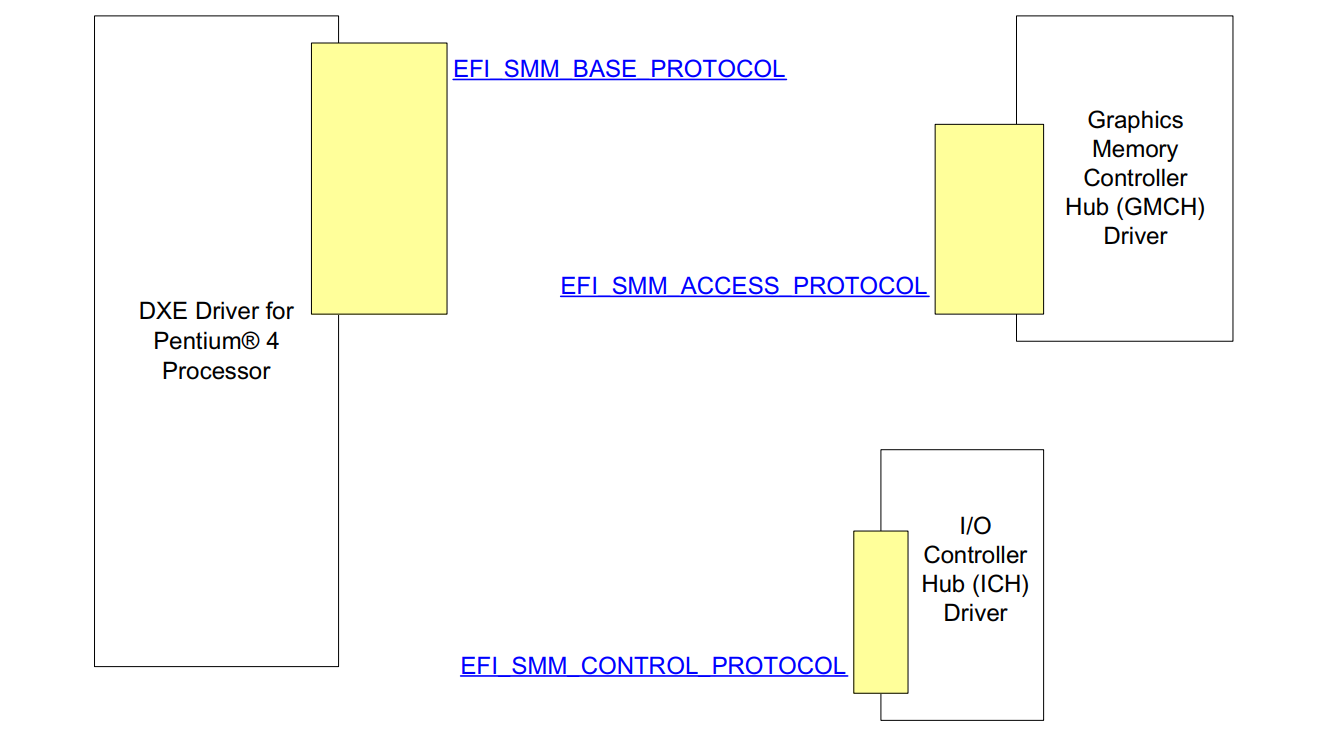
\includegraphics[width=0.9\linewidth]{smm/published-protocols-for-ia-32-systems}
	\caption{Protocols Published for IA-32 Systems}\label{fig:published-protocols-for-ia-32-systems}
\end{figure}

\subsubsection{SMM Protocols for "Itanium®-Based Systems"}
Figure \ref{fig:published-protocols-for-itanium-systems} shows the way SMM protocols are published for an \say{Itanium®-Based system}.
\begin{figure}[!htbp]
	\centering
	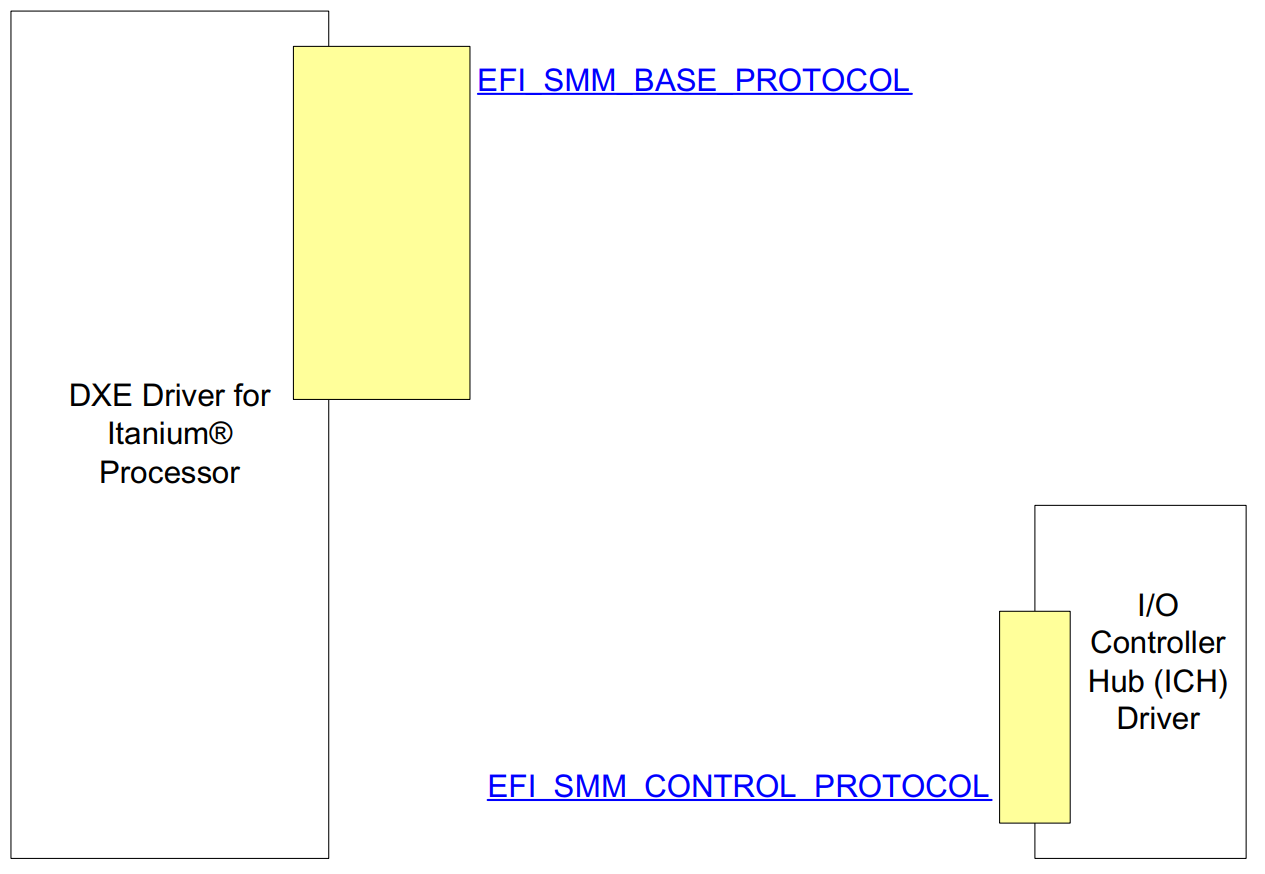
\includegraphics[width=0.9\linewidth]{smm/published-protocols-for-itanium-systems}
	\caption{Protocols Published for "Itanium®-Based Systems"}\label{fig:published-protocols-for-itanium-systems}
\end{figure}


\subsection{SMM Dispatcher and infrastructure}
SMM Code segment lies within the SMM Dispatcher. Major Role of SMM Dispatcher is to give the control mode to the SMM handlers in a systematic methodology. SMM Infrastructure Code aids to drive communication for SMM to SMM. SMM handlers are PE32+ images.

\subsection{Initializing SMM Phase}
The SMM driver for the Framework is fundamentally a enrollment transport mode to dispatch the drivers in outcome to the:
\begin{itemize}
	\item System Management Interrupts for \say{IA-32}
	\item Platform Management Interrupts (PMIs) for \say{Itanium® processor family}
\end{itemize}

\subsection{Relation of "System Management RAM (\gls{smram})" to conventional memory}
Figure \ref{fig:smram-relationship-to-main-memory} shows relationship between SMRAM and main memory in IA-32. Where SMRAM is isolated secure part inside the conventional main memory.

\begin{figure}[!htbp]
	\centering
	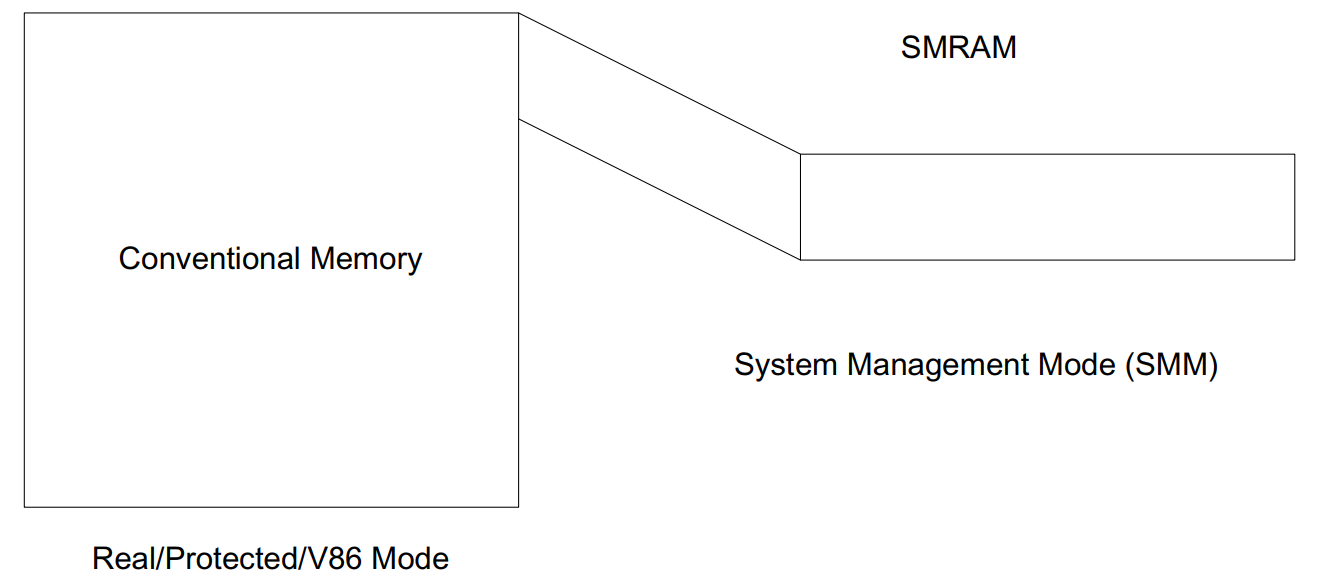
\includegraphics[width=0.9\linewidth]{smm/smram-relationship-to-main-memory}
	\caption{SMRAM kinship with conventional memory}\label{fig:smram-relationship-to-main-memory}
\end{figure}

\subsection{Execution Mode of SMM on Processor}\label{subsection-processor-execution-mode}
SMM is acceded asynchronously with the ongoing main flow of program. SMM was primitively developed to be clear to the OS and provide a power management facility more transparent.

Preboot agents are responsible to initiate alternate uses of SMM which are:
\begin{itemize}
	\item Applicable Workaround for \gls{soc} exaggeration
	\item Logging of error(s)
	\item Security for the platform
\end{itemize}

A \gls{smi} can be launched by energizing either the SMI logic pin via dedicated on the board or by utilizing the local APIC.

\say{Itanium® architecture} possess no independent separate mode for processor for the tractability of interruption however it does supports \say{Platform Management Interrupt (\gls{pmi})} which indeed is a maskable interruption. However, there is this another way to enter PMI using a interrupt message on local \say{Streamlined Advanced Programmable Interrupt Controller (\gls{sapic})}.

This architecture informs a techniques to load modules of needful code segment that substantiate the functionality specified above. The internal representation of protocol which enables the loading of images of various handler and runs in normal memory of boot-services. Only the handlers does to run in \gls{smram}.

\subsection{Accessing Platform Resources}\label{subsection-access-to-platform-resources}
As par policy outcome process of the execution of SMM handlers is reasonably prevents from accessing conventional memory resources. Hence, there does not exist any ease binding technique such as a call or trap interface to render the services in preemptive bid of non-SMM state.

Besides, SMM Services - the library of service which abides a sub set of the core EFI services, i.e. device input-output protocol, memory allocation and others. Also, execution mode of SMM driver has the equivalent structure as per the EFI criterion - namely a components which executes under boot services and it could perhaps run in runtime mode. When \verb|ExitBootServices()| invoked, the mechanism of an unregister event occurs.



